\section{Special Execution Platforms}
\label{sec:Execution_Platfors}

This section provides information about how to run COMPSs Applications in specific platforms such as \textit{Docker},
\textit{Chameleon} or \textit{MareNostrum}.


%%%%%%%%%%%%%%%%%%%%%%%%%%%%%%%%%%%%%%%%%
%% DOCKERS
%%%%%%%%%%%%%%%%%%%%%%%%%%%%%%%%%%%%%%%%%
\subsection{Docker}

\subsubsection{Introduction}
Docker is an open-source project that automates the deployment of applications inside software containers, 
by providing an additional layer of abstraction and automation of operating-system-level virtualization on Linux.
In addition to the Docker container engine, there are other Docker tools that allow users to create complex applications (Docker-Compose) 
or to manage a cluster of Docker containers (Docker Swarm).
\\ \\ 
COMPSs supports running a distributed application in a Docker Swarm cluster.
\\

\subsubsection{Requirements}
In order to use COMPSs with Docker, some requirements must be fulfilled:
\begin{itemize}  
\item Have \textbf{Docker} and \textbf{Docker-Compose} installed in your local machine.
\item Have an available \textbf{Docker Swarm cluster} and its Swarm manager ip and port to access it remotely.
\item A \textbf{Dockerhub account}. Dockerhub is an online repository for Docker images. We don't currently support
      another sharing method besides uploading to Dockerhub, so you will need to create a personal account.
      This has the advantage that it takes very little time either upload or download the needed images, since it 
      will reuse the existing layers of previous images (for example the COMPSs base image).
\end{itemize}


\subsubsection{Execution}

The runcompss-docker execution workflow uses Docker-Compose, which is in charge of spawning the different application containers into the Docker Swarm manager.
Then the Docker Swarm manager schedules the containers to the nodes and the application starts running.\\

The COMPSs master and workers will run in the nodes Docker Swarm decides. To see where the masters and workers are located in runtime,
you can use:
\begin{lstlisting} 
docker -H '<swarm_manager_ip:swarm_port>' ps -a 
\end{lstlisting}

The execution of an application using Docker containers with COMPSs \textbf{consists of 2 steps}:

\subsubsection{Execution step 1: Creation of the application image}
The very first step to execute a COMPSs application in Docker is creating your application Docker image. \\
This must be done \textbf{only once} for every new application, and then you can run it as many times as needed. 
If the application is updated for whatever reason, this step must be done again to create and share 
the updated image. \\
In order to do this, you must use the \textbf{compss\_docker\_gen\_image} tool, which is available in the standard COMPSs application.
This tool is the responsible of taking your application, create the needed image, and upload it to Dockerhub to share it. \\
The image is created injecting your application into a COMPSs base image. This base image is available in Dockerhub. 
In case you need it, you can pull it using the following command:
\begin{lstlisting}[language=bash]
docker pull compss/compss
\end{lstlisting}
The \textbf{compss\_docker\_gen\_image} script receives 2 parameters:
\begin{itemize}
 \item { 
 \textbf{-{}-c, -{}-context-dir:} \\ 
 Specifies the \textbf{context directory} path of the application. This path \textbf{MUST BE ABSOLUTE}, not relative.
 The context directory is a local directory that \textbf{must contain the needed binaries and input files of the app (if any)}.
 In its simplest case, it will contain the executable file (a .jar for example). Keep the context-directory as lightest as possible.
 
 For example: \textbf{-{}-context-dir='/home/compss-user/my-app-dir'} (where 'my-app-dir' contains 'app.jar', 'data1.dat' and 'data2.csv').
 For more details, this context directory will be recursively copied into a COMPSs base image. 
 Specifically, it will create all the path down to the context directory inside the image.
 }
 
 \item { 
 \textbf{-{}-image-name:} \\
 Specifies a name for the created image. It MUST have this format: 'DOCKERHUB-USERNAME/image-name'. \\
 The \textit{DOCKERHUB\_USERNAME} must be the username of your personal Dockerhub account. \\
 The \textit{image\_name} can be whatever you want, and will be used as the identifier for the image in Dockerhub.
 This name will be the one you will use to execute the application in Docker. \\
    For example, if my Dockerhub username is john123 and I want my image to be named "my-image-app": --image-name="john123/my-image-app".
 
 As stated before, this is needed to share your container application image with the nodes that need it.
 Image tags are also supported (for example "john123/my-image-app:1.23). 
 } 
\end{itemize}

\colorComment{\textbf{IMPORTANT NOTE:} \\ 
After creating the image, be sure to write down the absolute context-directory and the absolute classpath (the absolute path to the executable jar).
You will need it to run the application using \textbf{runcompss-docker}. In addition, if you plan on distributing the application,
you can use the Dockerhub image's information tab to write them, so the application users can retrieve them.}

 
\subsubsection{Execution step 2: Run the application}
To execute COMPSs in a Docker Swarm cluster, you must use the \textbf{runcompss-docker} command, instead of runcompss.
\\
The command \textbf{runcompss-docker} has some \textbf{additional arguments} that will be needed by COMPSs to run your application 
in a distributed Docker Swarm cluster environment.
The rest of typical arguments (classpath for example) will be delegated to runcompss command.
\\ \\
These additional arguments must go before the typical runcompss arguments. 
The runcompss-docker additional arguments are:
\begin{itemize}
 \item { 
 \textbf{-{}-w, -{}-worker-containers:} \\  
 Specifies the number of \textbf{worker containers} the app will execute on. One more container will be created to host the \textbf{master}. 
 If you have enough nodes in the Swarm cluster, each container will be executed by one node. This is the default schedule strategy used by Swarm. \\
 For example:  \textbf{-{}-worker-containers=3}
 }
 
 \item { 
 \textbf{-{}-s, -{}-swarm-manager:} \\
 Specifies the Swarm manager ip and port (format: ip:port). \\
 For example: \textbf{-{}-swarm-manager='129.114.108.8:4000'}
 }
 
 \item { 
 \textbf{-{}-i, -{}-image-name:} \\
 Specify the image name of the application image in Dockerhub. Remember you must generate this with compss\_docker\_gen\_image
 Remember as well that the format must be: 'DOCKERHUB\_USERNAME/APP\_IMAGE\_NAME:TAG' (the :TAG is optional). \\
 For example: \textbf{-{}-image-name='john123/my-compss-application:1.9'}
 }
                                 
 \item { 
 \textbf{-{}-c, -{}-context-dir:} \\
 Specifies the \textbf{context directory} of the app. It must be specified by the application image provider. \\
 For example: \textbf{-{}-context-dir='/home/compss-user/my-app-context-dir'}.
 }
\end{itemize}

As \textbf{optional} arguments:
\begin{itemize}
 \item { 
 \textbf{-{}-c-cpu-units:} \\
 Specifies the number of cpu units used by each container (default value is 4). \\
 For example: \textbf{-{}-c-cpu-units:=16}
 }
 
 \item { 
 \textbf{-{}-c-memory:} \\
 Specifies the physical memory used by each container in GB (default value is 8 GB).\\
 For example, in this case, each container would use as maximum 32 GB of physical memory: \textbf{-{}-c-memory=32}
 }
\end{itemize}

Here is the \textbf{format} you must use with \textbf{runcompss-docker} command:
\begin{lstlisting}[language=bash]
runcompss-docker --worker-containers=N
                 --swarm-manager='<ip>:<port>'
                 --image-name='DOCKERHUB_USERNAME/image_name'
                 --context-dir='CTX_DIR'
                 [rest of classic runcompss args]
\end{lstlisting}           

Or alternatively, in its shortest form:
\begin{lstlisting}[language=bash]
runcompss-docker --w=N --s='<ip>:<port>' --i='DOCKERHUB_USERNAME/image_name' --c='CTX_DIR'
                 [rest of classic runcompss args]
\end{lstlisting}        


\subsubsection{Execution with TLS}

If your cluster uses \textbf{TLS} or has been created using \textbf{Docker-Machine}, you will have to 
\textbf{export two environment variables} before using runcompss-docker:\\ \\

On one hand, \textbf{DOCKER\_TLS\_VERIFY} environment variable will tell Docker that you are using TLS:

\begin{lstlisting}[language=bash]
export DOCKER_TLS_VERIFY="1"
\end{lstlisting}
On the other hand, \textbf{DOCKER\_CERT\_PATH} variable will tell Docker where to find your TLS certificates. As an example:
\begin{lstlisting}[language=bash]
export DOCKER_CERT_PATH="/home/compss-user/.docker/machine/machines/my-manager-node"
\end{lstlisting}

In case you have created your cluster using docker-machine, in order to know what
your \textit{DOCKER\_CERT\_PATH} is, you can use this command:
\begin{lstlisting}[language=bash]
docker-machine env my-swarm-manager-node-name | grep DOCKER_CERT_PATH
\end{lstlisting}
In which \textit{swarm-manager-node-name} must be changed by the name docker-machine has assigned to your swarm manager node.\\ \\
With these environment variables set, you are ready to use \textbf{runcompss-docker} in a cluster using TLS.

\clearpage
\subsubsection{Execution results}
The execution results will be retrieved from the master container of your application.
\\ \\ 
If your context-directory name is \textbf{'matmul'}, then your results will be saved in the \textbf{'matmul-results'} directory, 
which will be located in the same directory you executed runcompss-docker on. 
\\ \\ 
Inside the \textbf{'matmul-results'} directory you will have:
\begin{itemize}
 \item {A folder named \textbf{'matmul'} with all the result files that were
	in the same directory as the executable when the application execution ended.  
	More precisely, this will contain the context-directory state right after finishing your application execution.
	\\
	\\
	Additionally, and for more advanced debug purposes,
	you will have some intermediate files created by runcompss-docker (Dockerfile, project.xml, resources.xml),
	in case you want to check for more complex errors or details. 
	}
	
  \item {A folder named \textbf{'debug'}, which (in case you used the runcompss debug option (\textbf{-d})), 
         will contain the \textbf{'.COMPSs'} directory, which contains another directory in which there are the typical debug files runtime.log, jobs, etc.
	 \\
         Remember \textbf{.COMPSs} is a \textbf{hidden} directory, take this into account if you do \textbf{ls} inside the debug directory (add the \textbf{-a} option).
  }
  
\end{itemize}

To make it simpler, we provide a \textbf{tree visualization} of an example of what your directories should look like after the execution.
In this case we executed the \textbf{Matmul example application} that we provide you:

~ \newline

\begin{figure}[!ht]
  \centering
    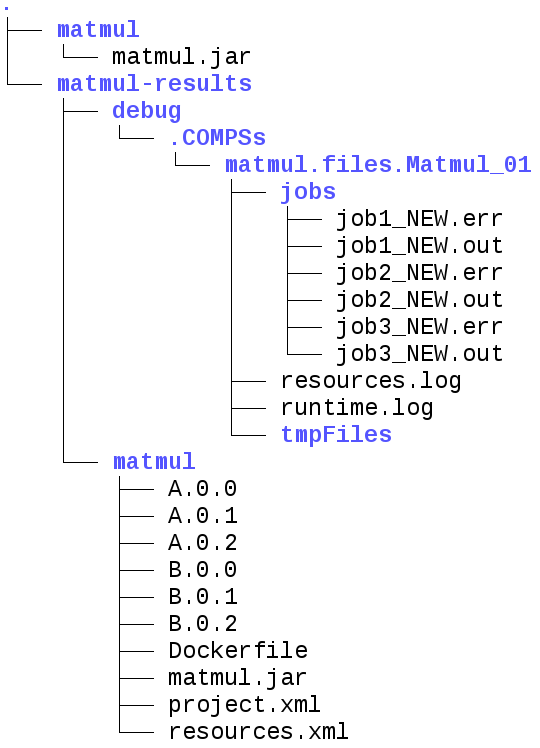
\includegraphics[width=0.3\textwidth]{./Sections/5_Execution_Platforms/Figures/docker-matmul-results-tree.png}
    \caption{Result and log folders of a \textit{Matmul} execution with COMPSs and Docker}
    \label{fig:compss_docker_results}
\end{figure}


\clearpage
\subsubsection{Execution examples}

  Next we will use the \textit{Matmul} application as an example of a Java application running with COMPSs and Docker.

Imagine we have our Matmul application in \texttt{/home/john/matmul} and inside the \texttt{matmul} directory we only have the file \texttt{matmul.jar}.

We have created a Dockerhub account with username 'john123'.

The first step will be creating the image:
\begin{lstlisting}[language=bash]
compss_docker_gen_image    --context-dir='/home/john/matmul'
			   --image-name='john123/matmul-example'
\end{lstlisting}

Now, we write down the context-dir (\texttt{/home/john/matmul}) and the classpath \\ (\texttt{/home/john/matmul/matmul.jar}). We do this because they will be needed for future executions. \\

Since the image is created and uploaded, we won't need to do this step anymore.

~ \newline

Now we are going to execute our Matmul application in a Docker cluster.

Take as assumptions:
\begin{itemize}  
\item We will use \textbf{5 worker docker containers}.
\item The \textbf{swarm-manager ip} will be 129.114.108.8, with the Swarm manager listening to the \textbf{port} 4000.
\item We will use \textbf{debug (-d)}.
\item Finally, as we would do with the typical runcompss, we specify the \textbf{main class} name and its \textbf{parameters} (16 and 4 in this case).
\end{itemize}

In addition, we know from the former step that the image name is \texttt{john123/matmul-example}, 
the \textbf{context directory} is \texttt{/home/john/matmul}, and the classpath is \texttt{/home/john/matmul/matmul.jar}.
And this is how you would run \textbf{runcompss-docker}:

\begin{lstlisting}[language=bash]
runcompss-docker --worker-containers=5
                 --swarm-manager='129.114.108.8:4000'
                 --context-dir='/home/john/matmul'
                 --image-name='john123/matmul-example'
                 --classpath=/home/john/matmul/matmul.jar
                 -d
                 matmul.objects.Matmul 16 4
\end{lstlisting}

Here we show another example using the short arguments form, with the KMeans example application, 
that is also provided as an example COMPSs application to you:

First step, create the image once:
\begin{lstlisting}[language=bash]
compss_docker_gen_image    --context-dir='/home/laura/apps/kmeans'
			   --image-name='laura-67/my-kmeans'
\end{lstlisting}

And now execute with 30 worker containers, and Swarm located in '110.3.14.159:26535'.
\begin{lstlisting}[language=bash]
runcompss-docker --w=30 --s='110.3.14.159:26535' --c='/home/laura/apps/kmeans' 
                 --image-name='laura-67/my-kmeans'
                 --classpath=/home/laura/apps/kmeans/kmeans.jar
                 kmeans.KMeans
\end{lstlisting}           

\clearpage

%%%%%%%%%%%%%%%%%%%%%%%%%%%%%%%%%%%%%%%%%
%% CHAMEMELON
%%%%%%%%%%%%%%%%%%%%%%%%%%%%%%%%%%%%%%%%%
\subsection{Chameleon}

\subsubsection{Introduction}

The Chameleon project is a configurable experimental environment for large-scale cloud research based on a \textit{OpenStack} 
KVM Cloud. With funding from the \textit{National Science Foundation (NSF)}, it provides a large-scale platform to the open research
community allowing them explore transformative concepts in deeply programmable cloud services, design, and core technologies. The 
Chameleon testbed, is deployed at the \textit{University of Chicago} and the \textit{Texas Advanced Computing Center} and consists of
650 multi-core cloud nodes, 5PB of total disk space, and leverage 100 Gbps connection between the sites. 

The project is led by the \textit{Computation Institute} at the \textit{University of Chicago} and partners from the \textit{Texas 
Advanced Computing Center} at the \textit{University of Texas} at Austin, the \textit{International Center for Advanced Internet 
Research} at \textit{Northwestern University}, the \textit{Ohio State University}, and \textit{University of Texas} at \textit{San
Antoni}, comprising a highly qualified and experienced team. The team includes members from the \textit{NSF} supported 
\textit{FutureGrid} project and from the \textit{GENI} community, both forerunners of the \textit{NSFCloud} solicitation under 
which this project is funded. Chameleon will also sets of partnerships with commercial and academic clouds, such as \textit{Rackspace},
\textit{CERN} and \textit{Open Science Data Cloud (OSDC)}.

For more information please check \url{https://www.chameleoncloud.org/} .

\subsubsection{Execution}

Currently, COMPSs can only handle the Chameleon infrastructure as a cluster (deployed inside a lease). Next, we provide the steps
needed to execute COMPSs applications at Chameleon:

\begin{itemize}
 \item Make a lease reservation with 1 minimum node (for the COMPSs master instance) and a maximum number of nodes equal to the
 number of COMPSs workers needed plus one
 \item Instantiate the master image (based on the published image \textit{COMPSs\_\compssversion\_CC-CentOS7})
 \item Attach a public IP and login to the master instance (the instance is correctly contextualized for COMPSs executions if you
 see a COMPSs login banner)
 \item Set the instance as COMPSs master by running \texttt{/etc/init.d/chameleon\_init start}
 \item Copy your CH file (API credentials) to the Master and source it
 \item Run the \texttt{chameleon\_cluster\_setup} script and fill the information when prompted (you will be asked for the name of the
 master instance, the reservation id and number of workers). This scripts may take several minutes since it sets up the all cluster.
 \item Execute your COMPSs applications normally using the \texttt{runcompss} script
\end{itemize}

As an example you can check this video \url{https://www.youtube.com/watch?v=BrQ6anPHjAU} performing a full setup and 
execution of a COMPSs application at Chameleon.


%%%%%%%%%%%%%%%%%%%%%%%%%%%%%%%%%%%%%%%%%
%% SuperComputers
%%%%%%%%%%%%%%%%%%%%%%%%%%%%%%%%%%%%%%%%%
\subsection{SuperComputers}

To maintain the portability between different environments, COMPSs has a pre-build structure (see Figure 
\ref{fig:queue_scripts_structure}) to execute applications in SuperComputers. For this purpose, users must use 
the \texttt{enqueue\_compss} script provided in the COMPSs installation. This script has several parameters (see 
\texttt{enqueue\_compss -h}) that allow users to customize their executions for any SuperComputer.

\begin{figure}[!ht]
  \centering
    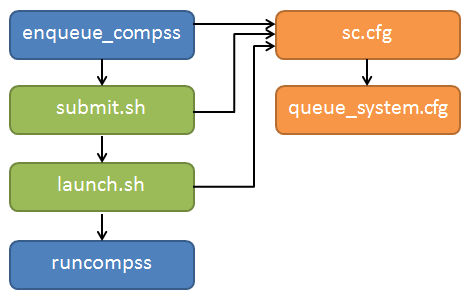
\includegraphics[width=0.6\textwidth]{./Sections/5_Execution_Platforms/Figures/queue_scripts_structure.png}
    \caption{Structure of COMPSs queue scripts. In Blue user scripts, in Green queue scripts and in Orange system dependant scripts}
    \label{fig:queue_scripts_structure}
\end{figure}

To make this structure works, the administrators must define a configuration file for the queue system and a configuration file
for the specific SuperComputer parameters. The COMPSs installation already provides queue configurations for \textit{LSF} and 
\textit{SLURM} and several examples for SuperComputer configurations. 
To create a new configuration we recommend to use one of the configurations provided by COMPSs (such as the configuration for the
\textit{MareNostrum IV} SuperComputer) or to contact us at \url{support-compss@bsc.es} .

~\newline

For information about how to submit COMPSs applications at any Supercomputer please refer to the \textit{COMPSs Supercomputers} manual 
available at \url{http://compss.bsc.es/releases/compss/latest/docs/COMPSs_Supercomputers_Manual.pdf} .
